\chapter{Metodologia}\label{cap:metodologia}

Este capítulo descreve as alterações introduzidas na \emph{baseline} do SoccerNet-GSR, nos módulos de reconhecimento do número da camisola e de atribuição da equipa e do lado do campo a cada jogador. Apresenta ainda a extensão do módulo de reidentificação com um descritor de cor, integrado para apoiar a atribuição da equipa.

Começa-se por situar estas alterações na arquitetura da \emph{baseline}, identificando os módulos alterados e os que se mantêm intactos. Segue-se a descrição do novo módulo de reconhecimento do número da camisola e dos módulos reescritos de atribuição da equipa e do lado do campo. Por fim, apresentam-se o ambiente experimental e o procedimento de avaliação em que assentam os resultados do capítulo seguinte.

\section{Visão Geral do Sistema}

A \emph{baseline} do SoccerNet-GSR é construída sobre o TrackLab \citep{joos2024tracklab}, um \emph{framework} \emph{open source} para o \emph{tracking} de múltiplos objetos, desenvolvido pelos autores da própria \emph{baseline}. O TrackLab organiza o processamento de um vídeo numa sequência de módulos, cada um responsável por uma etapa. Os módulos a executar, a sua ordem e os seus parâmetros são definidos em ficheiros de configuração, e os resultados de cada deteção ficam numa tabela comum, com uma linha por deteção, à qual cada módulo acrescenta os seus. Trocar um módulo por outro é, por isso, uma alteração de configuração que não obriga a mexer nos restantes. O TrackLab trata ainda do carregamento do conjunto de dados, da avaliação com a métrica oficial e da gravação dos resultados de cada vídeo, o que permite voltar a executar apenas os últimos módulos sem repetir os primeiros.

Os módulos são executados um de cada vez, e cada um processa o vídeo inteiro antes de o seguinte começar. Quando um módulo arranca, tem assim à sua disposição os resultados de todos os anteriores, para todas as imagens do vídeo. O que distingue os módulos é a quantidade de informação que cada um vê de cada vez, a que o TrackLab chama nível. Um módulo de nível imagem vê uma imagem de cada vez. Um módulo de nível deteção vê um recorte de cada vez, isto é, a região da imagem delimitada pela caixa de uma pessoa. Um módulo de nível vídeo vê de uma só vez todas as deteções do vídeo. A diferença tem consequências práticas. Um módulo que vê uma imagem ou um recorte de cada vez não consegue, por si só, relacionar o que acontece em imagens diferentes, enquanto um módulo de nível vídeo pode juntar todas as observações de um mesmo jogador ou comparar todos os jogadores entre si. A Figura~\ref{fig:pipeline-modulos} mostra os nove módulos da \emph{baseline} pela ordem em que são executados, com os de nível imagem ou deteção na linha de cima e os de nível vídeo na linha de baixo.

Os seis primeiros módulos produzem informação sobre cada deteção. O primeiro módulo (\texttt{bbox\_detector}) encontra as pessoas visíveis em cada imagem e delimita cada uma por uma caixa, a que se chama deteção. O detetor usado é o YOLOv8 \citep{jocher2023yolov8}. O segundo, a reidentificação (\texttt{reid}), descreve a aparência de cada deteção por um vetor de 256 números, construído de modo a que a mesma pessoa, vista em imagens diferentes, dê vetores parecidos. Estima também a função da pessoa, isto é, se é jogador, guarda-redes ou árbitro. O terceiro, o \emph{tracking} (\texttt{track}), feito pelo StrongSORT \citep{du2023strongsort}, usa a posição e o vetor de aparência para ligar as deteções da mesma pessoa em imagens consecutivas. Cada sequência de deteções assim ligadas forma um \emph{tracklet}, que representa o percurso de uma pessoa ao longo do vídeo, ou de parte dele.

O quarto e o quinto módulos tratam da geometria. A localização dos pontos do campo (\texttt{pitch}), feita pelo NBJW \citep{gutierrez2024nbjw}, encontra em cada imagem as linhas e as marcas notáveis do relvado. A calibração (\texttt{calibration}) usa-as para estimar a homografia, a transformação que leva cada ponto da imagem para o mapa do campo. Com ela, a posição dos pés de cada deteção passa a ser expressa em metros sobre o campo. O sexto, o reconhecimento do número da camisola (\texttt{jersey\_number\_detect}), tenta ler o número em cada recorte.

Os três últimos módulos trabalham sobre os \emph{tracklets} completos. A agregação (\texttt{tracklet\_agg}) junta as estimativas da função e as leituras do número de todas as deteções de um \emph{tracklet} e escolhe, por votação, uma função e um número para o \emph{tracklet} inteiro, de modo que uma leitura falhada numa imagem é corrigida pelas leituras das outras. A equipa (\texttt{team}) separa os \emph{tracklets} dos jogadores em dois grupos a partir da aparência. O lado do campo (\texttt{team\_side}) decide qual dos dois grupos defende a baliza da esquerda e qual defende a da direita, porque é assim, e não pelo nome ou pela cor, que a anotação do SoccerNet-GSR identifica as equipas. Estes dois módulos precisam de ver todos os jogadores do vídeo ao mesmo tempo, e por isso só podem ser de nível vídeo.

\begin{figure}[htbp]
    \centering
    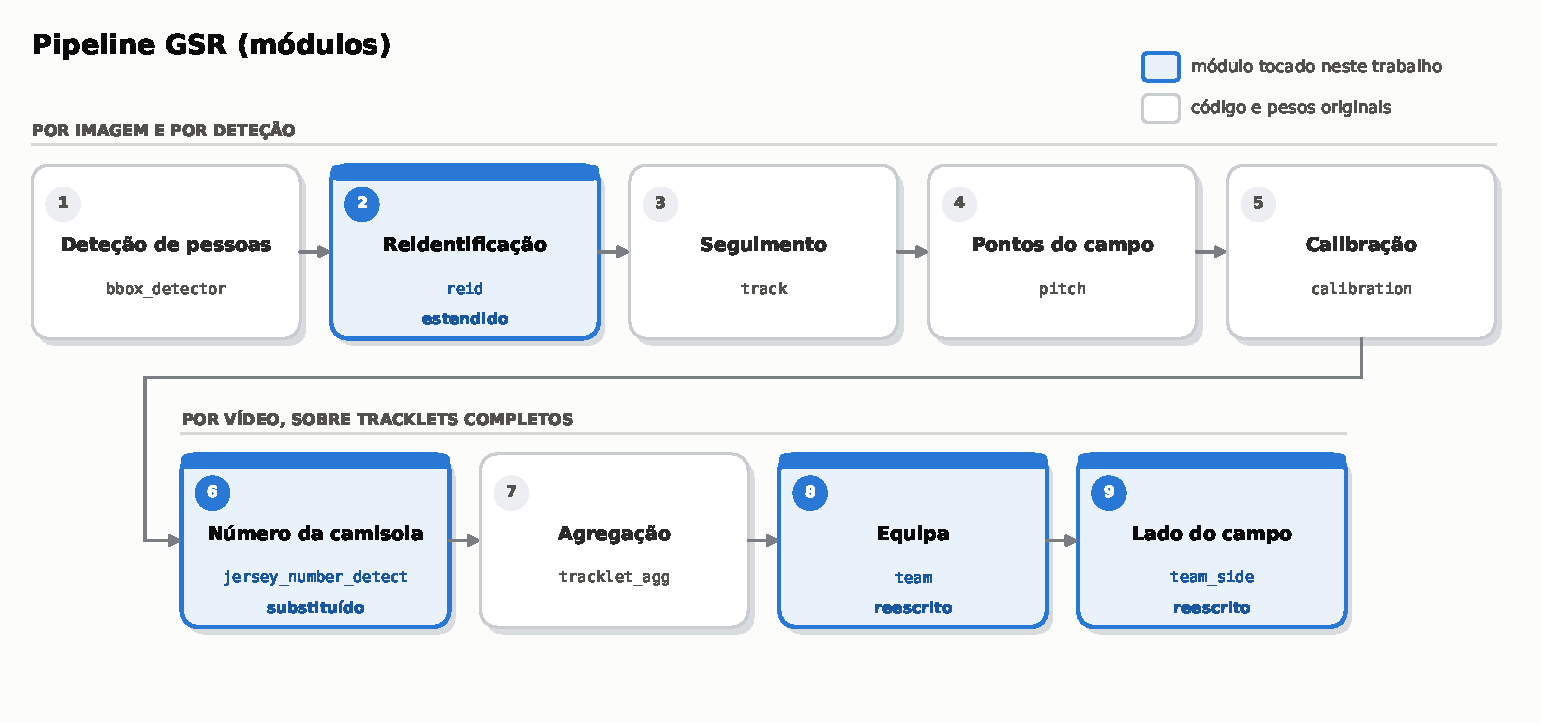
\includegraphics[width=\textwidth]{fig_pipeline_modulos.pdf}
    \caption{Os nove módulos do \emph{pipeline} da \emph{baseline}, pela ordem em que são executados. A azul, os quatro módulos em que este trabalho intervém. A reidentificação foi estendida com um descritor de cor, sem alterar o modelo nem o vetor de aparência original. O reconhecimento do número da camisola passou a ser feito por um módulo novo. O agrupamento em equipas e a atribuição do lado do campo foram reescritos. Os restantes cinco módulos correm com o código e os pesos originais.}
    \label{fig:pipeline-modulos}
\end{figure}

Este trabalho intervém em quatro dos nove módulos, assinalados a azul na Figura~\ref{fig:pipeline-modulos}. No reconhecimento do número da camisola (módulo 6), o MMOCR da \emph{baseline}, que lê cada recorte isoladamente, dá lugar a um modelo multimodal de visão e linguagem, descrito na Secção~\ref{sec:met-jnr}. O módulo continua a ser de nível deteção, mas guarda os recortes de cada \emph{tracklet} e só decide o número no fim do vídeo, quando o \emph{tracklet} está completo, o que lhe permite escolher as leituras em que confia. Os módulos da equipa e do lado do campo (módulos 8 e 9) são reescritos. O agrupamento passa a ser auditado e o lado passa a ser decidido por uma cascata de critérios, descritos na Secção~\ref{sec:met-equipa}. A reidentificação (módulo 2) é estendida sem ser alterada. O modelo e o vetor de aparência que o \emph{tracking} usa mantêm-se intactos, e acrescenta-se, para cada deteção, um descritor da cor do equipamento, que o módulo da equipa usa quando o vetor de aparência não chega para separar as equipas. Os restantes cinco módulos, a deteção, o \emph{tracking}, os pontos do campo, a calibração e a agregação, correm com o código e os pesos originais.

Os módulos alterados correspondem às lacunas identificadas na Secção~\ref{sec:sintese_lacunas}. O número da camisola é o atributo que mais custa ao GS-HOTA, tanto na \emph{baseline} como nos melhores sistemas do desafio. Entre os atributos de identificação, a equipa vem logo a seguir. O lado do campo, por sua vez, nunca tinha sido medido com \emph{tracklets} reais. Manter intactos os outros cinco garante que qualquer diferença de desempenho resulta das alterações introduzidas, e não de uma reotimização global do \emph{pipeline}. Como nenhuma das alterações exige treinar modelos, todas se integram na \emph{baseline} pública de \citet{somers2024soccernet} sem voltar a treinar as etapas anteriores.



\section{Reconhecimento do Número da Camisola}\label{sec:met-jnr}

Na \emph{baseline}, o reconhecimento do número da camisola é feito pela biblioteca MMOCR, que aplica um \emph{pipeline} genérico de deteção e reconhecimento de texto ao recorte do corpo inteiro de cada jogador. Como procura texto em todo o recorte, sem qualquer conhecimento prévio do domínio, esta abordagem trata o número como um texto qualquer e ignora duas propriedades do problema.

A primeira é espacial. O número encontra-se numa região anatomicamente delimitada, a zona dorsal do tronco, cuja localização pode ser estimada com precisão por um modelo de pose, em vez de ser procurada em todo o recorte. A segunda é temporal. O mesmo jogador é visto em muitas imagens consecutivas, mas o número só é legível em parte delas, por causa da baixa resolução, das oclusões e das poses desfavoráveis. Na \emph{baseline}, as leituras de todas as imagens são combinadas por votação simples, em que uma leitura nítida e uma leitura adivinhada valem o mesmo. Tirar partido desta redundância exige distinguir umas das outras.

Para aproveitar estas duas propriedades, o módulo proposto organiza o reconhecimento em três fases (Figura~\ref{fig:jnr-flow}). Primeiro, um modelo de estimativa de pose, o YOLO26m-pose \citep{jocher2026yolo26}, localiza os pontos do tronco (\emph{keypoints}) e isola a região dorsal, eliminando o fundo e as áreas irrelevantes do recorte. Depois, essa região é lida por um modelo multimodal de visão e linguagem (\emph{Vision-Language Model}, VLM), o Qwen2.5-VL \citep{bai2025qwen25vl}. O modelo interpreta a imagem no contexto do equipamento e distingue o número de outros elementos gráficos, como os patrocínios. Por fim, as leituras de cada \emph{tracklet} são combinadas numa decisão única, na qual só contam as leituras em que o próprio modelo indica estar seguro. As subsecções seguintes descrevem cada fase e justificam a escolha de cada modelo.


\begin{figure}[htbp]
    \centering
    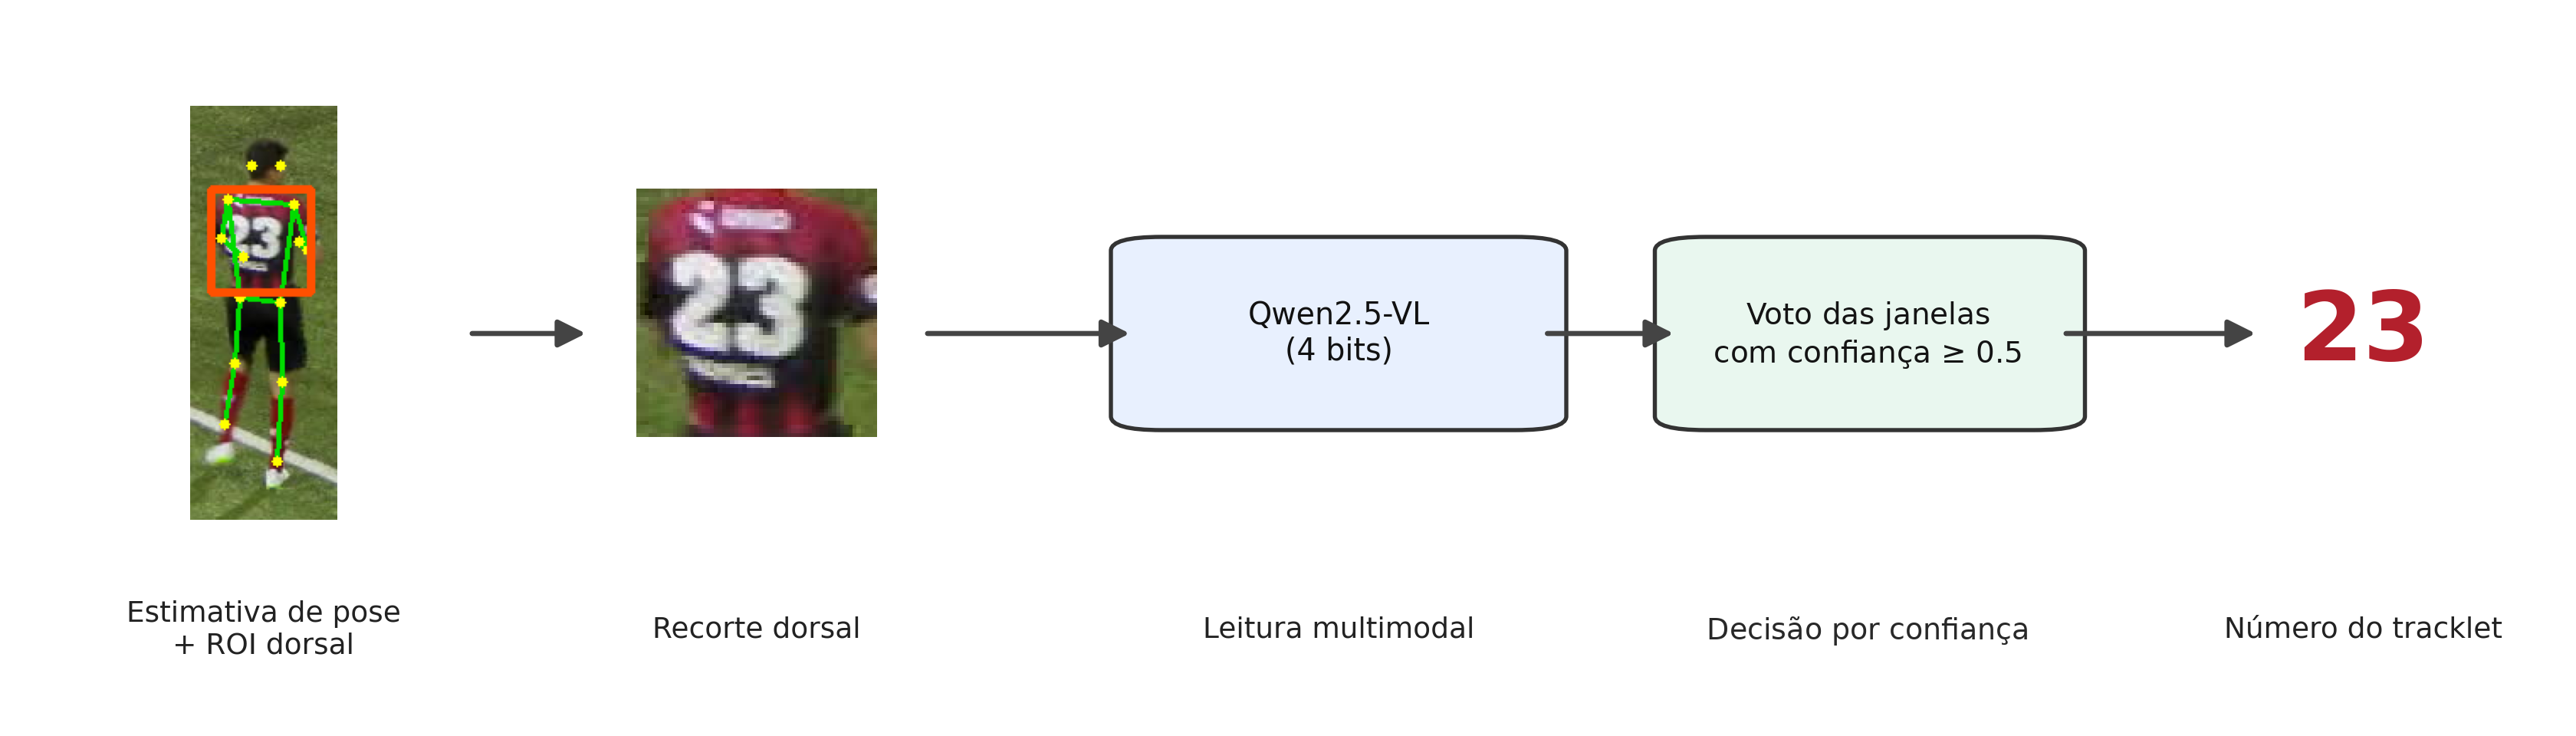
\includegraphics[width=\textwidth]{jnr_flow.png}
    \caption{Fluxo do módulo de reconhecimento do número da camisola. A estimativa de pose delimita a região dorsal, cujo recorte é interpretado pelo modelo multimodal Qwen2.5-VL quantizado a 4 bits. As leituras sucessivas de cada \emph{tracklet} são combinadas numa decisão final única, contando apenas as leituras com confiança suficiente.}
    \label{fig:jnr-flow}
\end{figure}

\subsection{Recorte da Região Dorsal por Estimativa de Pose}

Para concentrar a leitura na zona onde o número efetivamente aparece, cada deteção é primeiro processada por um modelo de estimativa de pose, o YOLO26m-pose. Usou-se a geração mais recente da família YOLO à data do trabalho, que sucedeu ao YOLOv11-pose das primeiras versões do módulo, na sua variante média, como compromisso entre a qualidade dos \emph{keypoints} e o tempo de execução, uma vez que o modelo corre sobre todas as deteções do vídeo. A partir dos \emph{keypoints} dos ombros e das ancas, define-se uma região de interesse sobre as costas do jogador, alargada lateralmente para acomodar variações de postura e enquadramento. O recorte é rejeitado quando o nariz ou um dos olhos é detetado com confiança superior a $0.6$, sinal de que o jogador está de frente para a câmara, ou quando os ombros e as ancas não são detetados com confiança suficiente. Esta regra simples foi a única filtragem da orientação que se manteve, depois de um classificador de orientação mais elaborado ter sido testado e descartado (Tabela~\ref{tab:alternativas}). O recorte final entrega ao modelo de leitura apenas a zona das costas, sem o fundo, os membros e a parte da frente.

Antes da leitura, cada recorte passa por um filtro de qualidade. São rejeitados os recortes com menos de $15\times20$ píxeis, tipicamente de jogadores muito distantes da câmara, e os recortes desfocados, cuja nitidez, medida pela variância do Laplaciano, fica abaixo de $15$. Estes limiares são baixos de propósito, para que o filtro elimine apenas os recortes claramente ilegíveis. Numa primeira versão do módulo, o filtro era a única defesa contra leituras de recortes sem informação, e os limiares tinham de ser altos ($25\times30$ píxeis e nitidez de $40$), o que excluía também jogadores cujo número era legível. Com a decisão pela confiança da leitura (Secção~\ref{sec:met-jnr-confianca}), é o próprio modelo que indica quando não conseguiu ler, e o filtro passa a servir apenas para evitar chamadas inúteis ao modelo.


\subsection{Leitura por Modelo Multimodal de Visão e Linguagem}

A leitura do número é feita pelo Qwen2.5-VL-3B-Instruct, um modelo multimodal de visão e linguagem (\emph{Vision-Language Model}, VLM) que recebe os recortes da região dorsal e devolve o número em texto. Preferiu-se um VLM a um motor de OCR dedicado porque o VLM interpreta o recorte no seu contexto. Distingue assim o número do jogador de outros elementos gráficos do equipamento, como patrocínios, logótipos ou textos avulsos, que um motor de OCR leria como texto e que introduziriam erros.

A principal restrição prática foi a memória da GPU, uma NVIDIA RTX~3060 portátil com 6~GB de VRAM partilhados com os restantes módulos. Em 16 bits, a precisão em que é distribuído, o Qwen2.5-VL-3B ocupa cerca de 7~GB e não cabe na GPU. Foi por isso carregado com quantização a 4 bits, através da biblioteca \emph{bitsandbytes}.

Quantizar um modelo é representar os seus pesos com menos bits do que os usados no treino, em troca de um pequeno erro de arredondamento \citep{gholami2021survey}. A \emph{bitsandbytes} fá-lo por blocos \citep{dettmers2023case, dettmers2023qlora}. Os pesos de cada camada linear são divididos em blocos de 64, e cada bloco é dividido pelo seu maior valor absoluto, que fica guardado em 32 bits como escala. Cada peso normalizado, agora entre $-1$ e $1$, é arredondado para o valor mais próximo do formato FP4, um número de vírgula flutuante de 4 bits, e é esse código de 4 bits que se guarda. Num bloco do próprio modelo, com escala $0.0510$, o peso $-0.0427$ dá $-0.837$ e fica guardado como $-1$. No cálculo, o código é multiplicado pela escala e convertido de novo para 16 bits. Cada peso passa a custar 4.5 bits em vez de 16, sem dados de calibração nem novo treino.

No Qwen2.5-VL-3B, as 414 camadas lineares são quantizadas no carregamento, com a configuração por omissão da biblioteca. Só a camada final, que produz as pontuações de cada \emph{token} usadas na Secção~\ref{sec:met-jnr-confianca}, fica em 16 bits. O modelo passa a ocupar 2.4~GB na GPU. O efeito da quantização na exatidão da leitura não foi medido, porque o modelo em 16 bits não cabe na GPU disponível.

O modelo é ainda libertado da GPU no fim de cada vídeo e recarregado no início do seguinte, para que os modelos dos pontos do campo e da calibração do vídeo seguinte, que correm antes do reconhecimento do número, não fiquem sem memória.

O \emph{prompt} dá ao modelo duas instruções. A primeira é ler o número inteiro. Sem ela, o modelo omite com frequência o primeiro algarismo quando este está parcialmente tapado, e lê, por exemplo, um 14 como 4. A segunda é não responder quando o recorte está pouco nítido, desfocado ou ambíguo, em vez de arriscar uma leitura incerta.

A política de recusa decorre da métrica. No GS-HOTA, um número errado nunca custa menos do que a ausência de resposta. Quando o jogador tem número anotado, os dois contam como erro. Quando não tem, só o número inventado é penalizado. É por isso preferível que o modelo não responda a que arrisque uma leitura incerta (Secção~\ref{sec:met-jnr-confianca}).

Para reduzir o número de chamadas ao modelo, a leitura feita durante a execução do \emph{pipeline} agrupa vários \emph{tracklets} na mesma chamada. Cada \emph{tracklet} entra como um grupo de recortes, identificado por um rótulo, e o modelo responde com uma linha por grupo, com o número ou com a indicação de que não o consegue ler. Cada chamada leva no máximo quatro \emph{tracklets} e vinte recortes, os mais nítidos de cada um. Este limite resultou de ensaios durante o desenvolvimento, nos quais a qualidade das respostas caía quando o modelo recebia mais de 15 a 20 imagens de uma vez. Os primeiros recortes de cada \emph{tracklet} são lidos numa chamada à parte. Juntá-los nessa fase a imagens de qualidade muito diferente levava o modelo a recusar a leitura de todos os grupos, mesmo dos que tinham o número visível. A leitura usada na decisão final é feita à parte, sobre conjuntos de recortes consecutivos, as janelas descritas na secção seguinte.

\subsection{Confiança da Leitura e Decisão por Janela}\label{sec:met-jnr-confianca}

A leitura efetuada sobre um recorte isolado é, por natureza, ruidosa. Uma pose desfavorável, uma oclusão momentânea ou variações de iluminação bastam para levar a uma leitura errada num \emph{frame}, mesmo quando o número se mantém legível na maior parte do \emph{tracklet} (Figura~\ref{fig:jnr-crops}). A decisão final tem, por isso, de combinar várias leituras, e a forma de as combinar determina o tipo de erro que o sistema comete.

\begin{figure}[H]
    \centering
    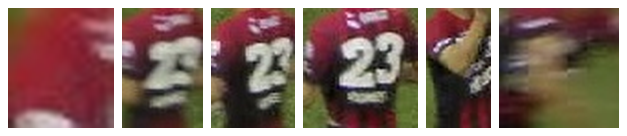
\includegraphics[width=0.9\textwidth]{jnr_crops_tracklet71.png}
    \caption{Recortes da região dorsal de um mesmo \emph{tracklet} ao longo do tempo. O número do jogador é nítido apenas em parte dos \emph{frames}. Esta variabilidade justifica decidir o número apenas com as leituras em que o modelo indica estar seguro.}
    \label{fig:jnr-crops}
\end{figure}

Para cada \emph{tracklet}, os recortes da região dorsal que passam o filtro de qualidade são ordenados no tempo e agrupados em janelas de seis recortes consecutivos, e cada janela dá origem a uma leitura (Figura~\ref{fig:jnr-janelas}). Para essa leitura escolhem-se os cinco recortes mais nítidos da janela, medidos pela variância do Laplaciano, que são apresentados em conjunto ao Qwen2.5-VL numa única chamada, com o \emph{prompt} descrito na secção anterior. A resposta é gerada com descodificação determinística (\emph{greedy decoding}), em que o modelo escreve, em cada passo, o \emph{token} mais provável, sem amostragem aleatória, pelo que a mesma janela produz sempre a mesma resposta. O modelo responde com um número ou recusa a leitura.

A confiança da leitura obtém-se da própria resposta. O Qwen2.5-VL escreve os números um dígito de cada vez, e cada dígito é um \emph{token} ao qual o modelo atribui uma probabilidade que mede a sua segurança. A confiança da janela é o produto das probabilidades dos dígitos do número. Para o número 14 lido com probabilidade $0.97$ no primeiro dígito e $0.93$ no segundo, a confiança é $0.97 \times 0.93 \approx 0.90$. Existe, assim, uma única confiança por janela, calculada sobre a resposta e não sobre cada recorte. Um número lido com segurança tem confiança próxima de $1$, enquanto um número adivinhado num recorte pouco legível fica muito abaixo, porque basta a incerteza num dos dígitos para baixar o produto.

\begin{figure}[H]
    \centering
    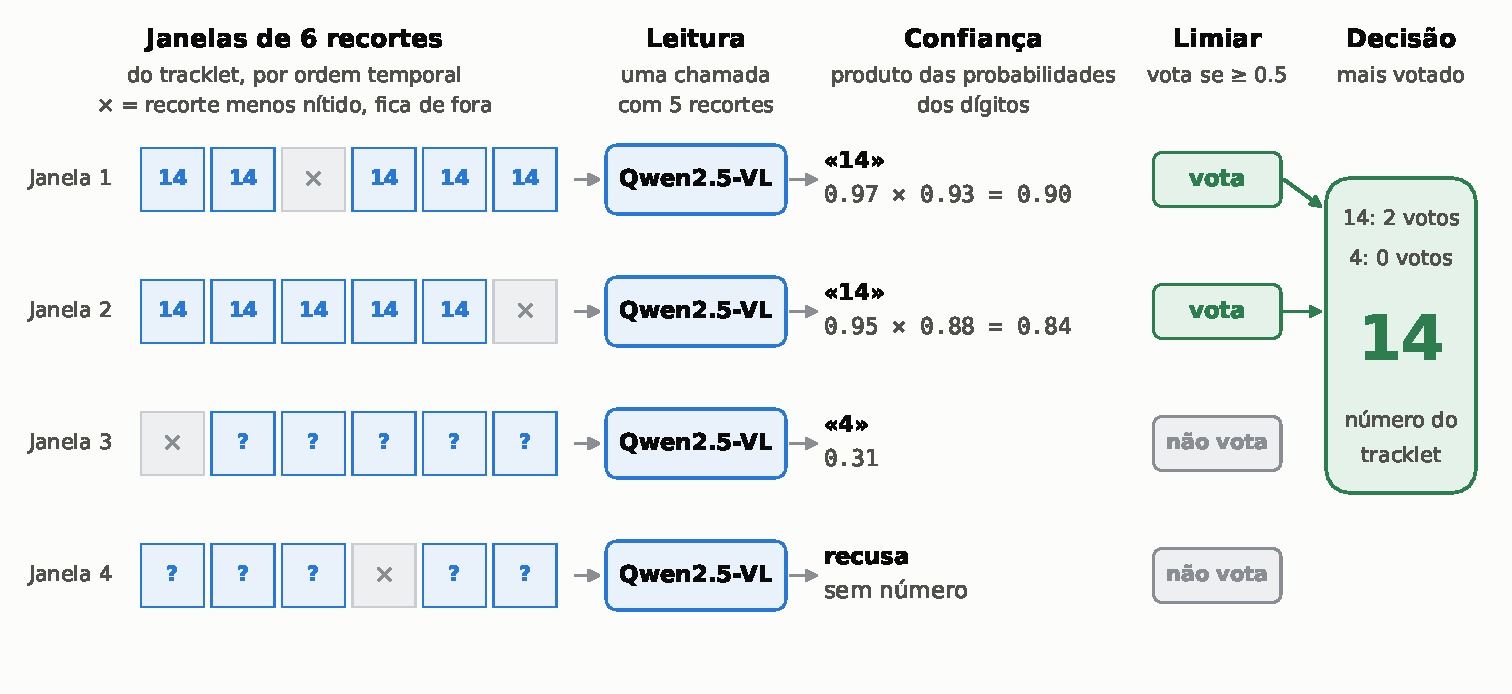
\includegraphics[width=\textwidth]{fig_jnr_janelas.pdf}
    \caption{Decisão do número de um \emph{tracklet} por janelas. Os recortes são agrupados em janelas de seis, e os cinco mais nítidos de cada janela são lidos numa única chamada ao Qwen2.5-VL. Nas janelas 3 e 4, o «?» marca os recortes em que o número não se lê. A confiança de cada leitura é o produto das probabilidades dos seus dígitos. Só votam as janelas com confiança igual ou superior a $0.5$, e o \emph{tracklet} recebe o número mais votado.}
    \label{fig:jnr-janelas}
\end{figure}

No fim do \emph{tracklet}, as leituras de todas as janelas são combinadas por votação, com duas regras. Uma janela só vota se tiver lido um número com confiança igual ou superior a $0.5$, pelo que não votam as janelas com confiança inferior nem aquelas em que o modelo recusou a leitura. O \emph{tracklet} recebe o número mais votado entre as janelas que votaram e, se nenhuma votou, fica sem número. A confiança decide, assim, que leituras contam, e a maioria decide o número.

Esta regra resulta de um diagnóstico realizado no próprio módulo. Na primeira versão, a função que chamava o modelo devolvia sempre a mesma confiança fixa, independentemente da certeza da leitura, e a decisão dependia apenas da contagem de votos, com uma quota mínima de concordância entre as janelas. Um número nítido e um número adivinhado, num recorte desfocado, pesavam o mesmo. Quando um jogador era visto durante muito tempo em más condições, as leituras erradas acumulavam votos suficientes para vencer, e o erro propagava-se a centenas de deteções. A confiança do modelo já existia, mas era descartada. Usá-la permite separar as leituras seguras das restantes antes da votação, em vez de tentar compensar a posteriori com quotas de concordância.

O limiar de 0.5 traduz uma escolha de projeto. Na métrica do SoccerNet-GSR, errar o número nunca custa menos do que deixá-lo em branco, e é pior quando o jogador não o tem anotado. Fora da métrica, a diferença é ainda maior. Um número errado dá ao jogador a identidade de outro, e a ausência de resposta apenas a deixa por atribuir. Entre errar e abster-se, o sistema foi desenhado para se abster. O custo desta escolha, medido no Capítulo~\ref{cap:resultados}, é um ligeiro aumento dos jogadores que ficam sem número.


\subsection{Alternativas Consideradas}

A solução final para a leitura do número não foi imediata. Antes de se chegar ao Qwen2.5-VL-3B, testaram-se abordagens de quatro tipos. O primeiro foi o de outros motores de OCR, como o EasyOCR \citep{jaidedai2020easyocr}, o PaddleOCR \citep{li2022ppocrv3} e o HunyuanOCR \citep{hunyuan2025ocr}. O segundo foi a versão maior do mesmo modelo, o Qwen2.5-VL-7B, com 7 mil milhões de parâmetros em vez de 3 mil milhões. O terceiro foi ampliar os recortes por super-resolução, com o Real-ESRGAN \citep{wang2021realesrgan}, antes de os ler. O quarto foram duas formas de pôr de parte os recortes em que o jogador não está de costas. Uma usava a reconstrução tridimensional do corpo pelo SAM 3D Body \citep{yang2026sam3dbody}, e a outra um classificador de orientação.

\begin{table}[htbp]
\centering
\caption{Alternativas consideradas para a leitura do número e motivo por que foram postas de parte.}
\label{tab:alternativas}
\renewcommand{\arraystretch}{1.35}
\setlength{\tabcolsep}{6pt}
\begin{tabular}{|p{3.6cm}|p{9.0cm}|}
\hline
\textbf{Abordagem} & \textbf{Razão do descarte} \\
\hline
EasyOCR e OCR clássico &
Mesma limitação estrutural do MMOCR, falha em números pequenos ou inclinados e não
distingue o número de outros elementos gráficos. \\
\hline
PaddleOCR (com \emph{fine-tuning}) &
Falha de segmentação (\emph{segfault}) ao inicializar no mesmo processo que o CUDA do
\emph{pipeline}, e mesmo isolado não recuperou leituras face ao Qwen. \\
\hline
HunyuanOCR &
\emph{VLM} mais pesado, sem ganho de exatidão que compensasse o custo de VRAM e de
latência no \emph{hardware} disponível. \\
\hline
Qwen2.5-VL-7B &
Requer cerca de 10\,GB de VRAM, acima dos 6\,GB da GPU, o que inviabiliza a sua
utilização. \\
\hline
Super-resolução (\mbox{Real-ESRGAN}) &
A informação em falta não existe na imagem de origem, e a ampliação amplifica o ruído
em vez de a recuperar. \\
\hline
SAM 3D Body &
Reconstrução tridimensional do corpo demasiado pesada para correr por \emph{frame} e
desadequada a um simples sinal de orientação. \\
\hline
Classificador de orientação &
O ganho de filtrar os \emph{frames} sem as costas visíveis não compensou, pois a votação
por \emph{tracklet} já absorve naturalmente esses \emph{frames}. \\
\hline
\end{tabular}
\end{table}


Estas experiências convergem numa conclusão. Em condições de baixa resolução, o fator decisivo não é a escolha do motor de OCR mais potente, mas sim entregar ao modelo a imagem certa, o recorte da região dorsal obtido por pose, e agregar bem as leituras ao longo do tempo. O Qwen2.5-VL-3B foi escolhido pelo equilíbrio entre exatidão e ocupação de memória, e não por ser o modelo de maior dimensão.


\section{Atribuição da Equipa e do Lado do Campo}\label{sec:met-equipa}

A atribuição da equipa divide-se em dois problemas distintos. O primeiro consiste em separar os \emph{tracklets} dos jogadores em dois grupos, um por equipa. O segundo consiste em determinar qual dos grupos defende a baliza da esquerda e qual defende a da direita. Este segundo passo é necessário porque a anotação do SoccerNet-GSR identifica as equipas pelo lado do campo que defendem, \emph{left} ou \emph{right}, e não pelo nome ou pela cor do equipamento. Um erro em qualquer dos dois problemas conta como erro na atribuição da equipa.

A \emph{baseline} resolve os dois problemas de forma simples. No primeiro, calcula para cada \emph{tracklet} de jogador a média das suas características de reidentificação, um vetor de 256 dimensões produzido pelo PRTreID, e agrupa esses vetores com um \emph{k-means} de dois grupos. O \emph{k-means} é um algoritmo de agrupamento não supervisionado que reparte as observações num número fixo de grupos. Cada observação é atribuída ao centro mais próximo e os centros são recalculados até a partição estabilizar. No segundo problema, a solução calcula a média da coordenada horizontal no campo de todas as deteções de cada grupo e declara \emph{right} o grupo com a média mais à direita. Os guarda-redes ficam fora do agrupamento e recebem, em cada deteção, o lado correspondente à metade do campo em que se encontram. Nenhum destes resultados é auditado. Se o \emph{k-means} misturar as equipas, os \emph{tracklets} mal agrupados ficam com a equipa errada. Se a média das posições apontar para o lado errado, todos os jogadores do vídeo ficam com o lado trocado.

Foi isso que a inspeção visual da \emph{baseline} mostrou, como o Capítulo~\ref{cap:resultados} quantifica. Nos $159$ vídeos, as falhas do próprio módulo de equipa repartem-se entre o agrupamento, com $14$ vídeos de equipas misturadas e $7$ colapsados numa só equipa, e o mapeamento para os lados, com $7$ vídeos de lado trocado. O lado trocado é a falha mais grave, porque deixa a $0\%$ todos os \emph{tracklets} do vídeo, mesmo quando os dois grupos estão corretos. Outros $20$ vídeos falham antes do agrupamento, no classificador de função, que este trabalho não alterou. As alterações descritas a seguir atuam por isso nas duas fases do processo, mas de forma diferente. No agrupamento, mantém-se o método original e acrescenta-se uma auditoria que, quando o resultado é pouco fiável, recorre a um agrupamento alternativo pela cor do equipamento. Esta alternativa exige um descritor novo, calculado no módulo de reidentificação. No mapeamento para os lados, substitui-se a comparação de médias por uma cascata de quatro critérios, em que essa comparação passa a ser o último recurso.

\subsection{Descritor de Cor do Equipamento}\label{sec:descritor-cor}

Para separar as equipas, a \emph{baseline} usa o vetor de $256$ números com que o PRTreID descreve a aparência de cada jogador. Este vetor foi treinado sobretudo para reconhecer o mesmo jogador ao longo do vídeo, e não para agrupar os jogadores por equipa. Por isso mistura a cor do equipamento com outros traços, como a forma do corpo, a pose ou o cabelo. Quando os equipamentos das duas equipas são parecidos, ou quando a imagem é pequena ou mal iluminada, dois jogadores de equipas diferentes podem ficar tão próximos como dois jogadores da mesma equipa, e o agrupamento mistura as equipas.

Para dispor de um sinal que dependa apenas da cor da camisola, acrescentou-se ao módulo de reidentificação um descritor de cor, calculado para cada deteção. O descritor tem $27$ números e é construído em três passos, ilustrados na Figura~\ref{fig:descritor-cor}. Primeiro, isolam-se os píxeis da camisola. Depois, descreve-se a cor desses píxeis. Por fim, guarda-se o resultado ao lado do vetor original, sem o alterar.

\begin{figure}[H]
    \centering
    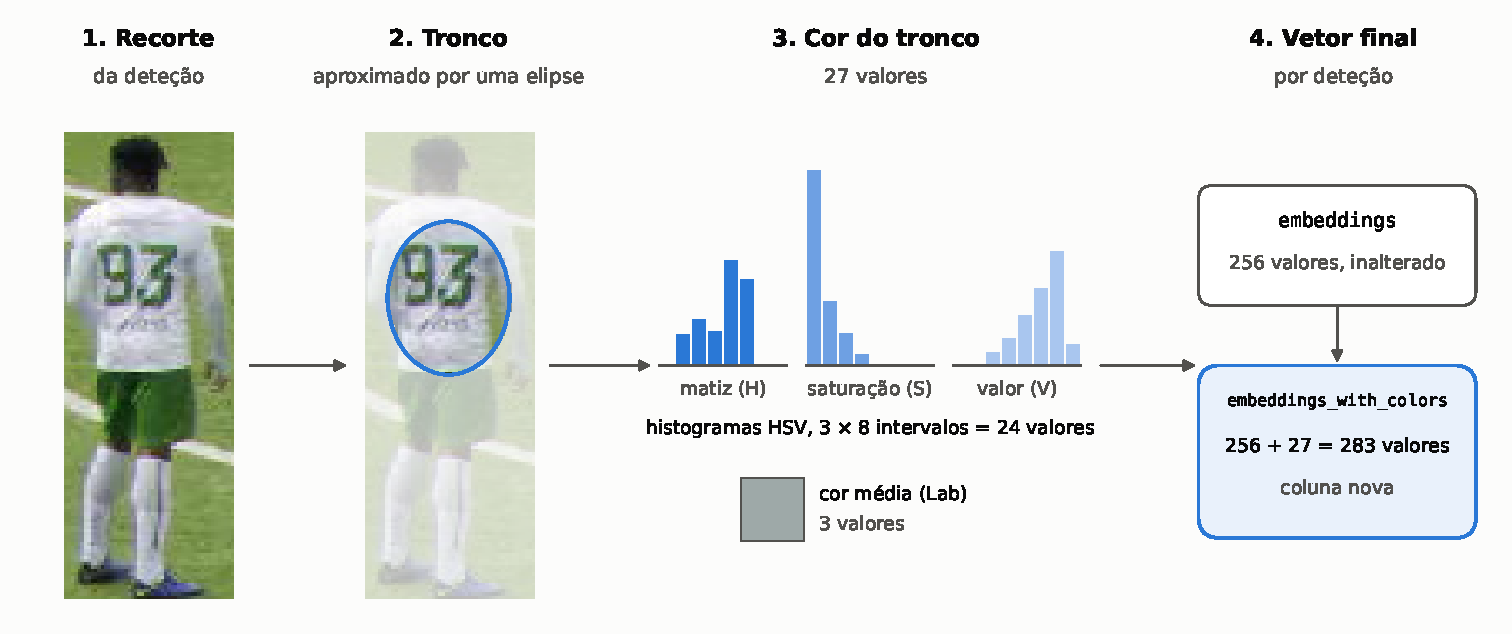
\includegraphics[width=\textwidth]{fig_descritor_cor.pdf}
    \caption{Construção do descritor de cor para uma deteção do vídeo SNGS-116, do recorte da deteção ao vetor final guardado na coluna nova.}
    \label{fig:descritor-cor}
\end{figure}

Para isolar a camisola aproveita-se um resultado que o PRTreID já calcula. O modelo divide o corpo em seis partes, a cabeça, o tronco, os dois braços e as duas pernas, e produz para cada deteção um mapa que indica onde está cada parte. Usam-se apenas os píxeis em que o mapa do tronco atinge pelo menos $25\%$ do seu valor máximo, o que deixa de fora a relva, a pele, os calções e as meias. Nas deteções muito pequenas ou cortadas, em que o tronco reúne menos de $16$ píxeis, usa-se em alternativa a faixa central do recorte, entre $25\%$ e $75\%$ da altura. Como o mapa não é guardado, a Figura~\ref{fig:descritor-cor} representa o tronco por uma elipse.

A cor dos píxeis do tronco é descrita no espaço HSV, que representa cada píxel por três valores. A matiz indica a cor propriamente dita, como o vermelho ou o azul. A saturação indica se a cor é viva ou acinzentada, e o valor se é clara ou escura. São estes dois últimos canais que distinguem os equipamentos brancos, pretos ou cinzentos, que não têm matiz definida. Para cada canal, a escala de valores possíveis é dividida em oito intervalos iguais, cada píxel da camisola cai num desses intervalos e conta-se a fração dos píxeis que cai em cada um. Os três canais dão assim $3 \times 8 = 24$ números, que a Tabela~\ref{tab:hsv-exemplo} mostra para a camisola branca da Figura~\ref{fig:descritor-cor}. Saturação baixa e valor alto é o que caracteriza uma camisola branca. Juntam-se mais três números, a cor média dos mesmos píxeis no espaço Lab, um espaço em que a distância entre duas cores acompanha a diferença que o olho humano percebe.

\begin{table}[H]
    \centering
    \definecolor{azultab}{HTML}{2A78D6}
    \caption{Histograma HSV da camisola da Figura~\ref{fig:descritor-cor}, calculado sobre os $1336$ píxeis do tronco. Cada valor é a fração dos píxeis que cai em cada intervalo, do mais baixo ($1$) ao mais alto ($8$). Quanto mais escura a célula, maior a fração.}
    \label{tab:hsv-exemplo}
    \small
    \setlength{\tabcolsep}{4pt}
    \begin{tabular}{|l|c|c|c|c|c|c|c|c|l|}
        \hline
        \textbf{Canal} & \textbf{1} & \textbf{2} & \textbf{3} & \textbf{4} & \textbf{5} & \textbf{6} & \textbf{7} & \textbf{8} & \textbf{Leitura} \\
        \hline
        Matiz (H) & $0.00$ & \cellcolor{azultab!9}$0.10$ & \cellcolor{azultab!13}$0.15$ & \cellcolor{azultab!9}$0.11$ & \cellcolor{azultab!30}$0.35$ & \cellcolor{azultab!24}$0.28$ & $0.00$ & $0.00$ & Pouco fiável no branco \\
        \hline
        Saturação (S) & \cellcolor{azultab!55}$0.64$ & \cellcolor{azultab!18}$0.21$ & \cellcolor{azultab!9}$0.11$ & \cellcolor{azultab!3}$0.04$ & $0.00$ & $0.00$ & $0.00$ & $0.00$ & Baixa, sem cor viva \\
        \hline
        Valor (V) & $0.00$ & $0.00$ & \cellcolor{azultab!3}$0.04$ & \cellcolor{azultab!8}$0.09$ & \cellcolor{azultab!15}$0.17$ & \cellcolor{azultab!22}$0.26$ & \cellcolor{azultab!33}$0.38$ & \cellcolor{azultab!6}$0.07$ & Alto, cor clara \\
        \hline
    \end{tabular}
\end{table}

Os $27$ números são acrescentados aos $256$ do PRTreID e guardados numa coluna nova, \texttt{embeddings\_\allowbreak with\_\allowbreak colors}, com $283$ valores. A coluna original, \texttt{embeddings}, fica igual, e por isso o \emph{tracking}, que a usa, funciona exatamente como na \emph{baseline}. Só o agrupamento em equipas lê a coluna nova, e dela usa apenas os $27$ números de cor. Os casos em que o agrupamento recorre a estes números são descritos na Secção~\ref{sec:agrupamento}, e o efeito no resultado é medido na Secção~\ref{sec:res_equipa_ablacao}.

\subsection{Agrupamento em Duas Equipas com Auditoria}\label{sec:agrupamento}

O \emph{k-means} divide os \emph{tracklets} de jogador em dois grupos, um por equipa, e é a esta divisão que se chama agrupamento. Devolve sempre dois grupos, mesmo quando as características que recebe não separam as equipas, e a \emph{baseline} aceita o resultado sem o verificar. O módulo reescrito parte do mesmo agrupamento, mas submete-o a duas verificações antes de o aceitar. A primeira, «Separação clara?», verifica se os dois grupos estão bem separados no espaço de reidentificação. Se não estiverem, o agrupamento é refeito com o descritor de cor da Secção~\ref{sec:descritor-cor}, e o novo agrupamento só é usado se passar a verificação «Cor aceite?». A segunda, «Duas equipas?», verifica se o agrupamento que sai da primeira tem, de facto, duas equipas. Se não tiver, os \emph{tracklets} são reagrupados pela cor medida diretamente nas imagens, e este agrupamento de resgate só é usado se passar a verificação «Resgate aceite?». Sempre que uma alternativa é recusada, mantém-se o agrupamento que vinha de trás. Quando nenhuma verificação falha, o agrupamento final é o da reidentificação, como na \emph{baseline}.

O primeiro passo é o da \emph{baseline}. Para cada \emph{tracklet} de jogador calcula-se a média de três grandezas ao longo das suas deteções, o vetor de reidentificação de $256$ números, o descritor de cor de $27$ números e a posição horizontal no campo. Esta posição é a coordenada $x$ dos pés do jogador no mapa do campo, que a calibração exprime em metros, com origem no centro. Como o campo do SoccerNet-GSR tem $105$ metros de comprimento, $x$ vai de $-52.5$ metros, na linha de baliza da esquerda, a $+52.5$ metros, na da direita. Uma deteção com $|x|$ acima de $52.5$ metros fica para lá da linha de baliza, o que num jogador em campo resulta quase sempre de uma falha pontual da calibração, capaz de projetar os pés a centenas de metros. Essas deteções são ignoradas, porque uma só bastaria para deslocar a média do \emph{tracklet}, e a média só é calculada se restarem pelo menos três deteções. Os vetores de reidentificação são então agrupados com um \emph{k-means} de dois grupos, que corre dez vezes com centros iniciais diferentes e fica com o resultado mais compacto, para que não dependa de um mau ponto de partida. A cor e a posição ainda não entram nesta fase e só são usadas nas verificações descritas a seguir, a posição para saber em que metade do campo está cada \emph{tracklet}. A reidentificação é, portanto, o sinal principal. Na maioria dos vídeos é ela que separa as equipas, e a cor só é chamada quando essa separação não é fiável.


A decisão «Separação clara?» usa duas medidas. A primeira é o coeficiente de silhueta. Para cada \emph{tracklet}, compara-se a distância média aos \emph{tracklets} do seu grupo com a distância média aos do outro grupo, o que dá um valor entre $-1$ e $1$. Perto de $1$, os grupos são compactos e afastados, como se espera de duas equipas com equipamentos diferentes. Perto de zero, sobrepõem-se e a divisão pode ser arbitrária. A segunda medida é a distância entre os centros dos dois grupos no espaço de reidentificação. A separação é dada como pouco clara em dois casos. No primeiro, a silhueta média fica abaixo de $0.28$. No segundo, herdado de uma versão anterior do módulo, pelo menos $85\%$ dos \emph{tracklets} estão na mesma metade do campo e os centros distam menos de $2.04$. Nesses vídeos a posição dos jogadores pouco ajuda a decidir o lado, e um erro de agrupamento sai mais caro.

O valor de $2.04$ não tem significado geral e deve ser lido como tal. Nos quatro vídeos de teste em que o segundo caso se verifica, a distância entre centros foi de $1.799$, $1.896$, $1.981$ e $2.035$, e o limiar ficou $0.005$ acima do maior destes valores. Manteve-se porque retirá-lo introduzia regressões no conjunto de teste. O primeiro caso foi acrescentado mais tarde, calibrado sobre os conjuntos de teste e de validação em conjunto, precisamente para cobrir os vídeos em que a jogada não se concentra numa metade e o segundo caso nunca se verifica.

Quando a separação não é clara, o \emph{k-means} é repetido sobre os $27$ números do descritor de cor, normalizados para que cada um tenha média zero e desvio-padrão um. A cor é usada sozinha, e não junta aos $256$ números da reidentificação, porque depois da normalização todos os números pesam o mesmo e os $256$ da reidentificação abafariam os $27$ da cor. A decisão «Cor aceite?» exige que o grupo menor do agrupamento por cor reúna pelo menos $20\%$ dos \emph{tracklets}. Abaixo disso, o \emph{k-means} terá isolado um punhado de \emph{tracklets} atípicos, com sombra ou oclusão, e não as duas equipas, e mantém-se o agrupamento por reidentificação. Esta exigência só se aplica ao primeiro caso. No segundo, o agrupamento por cor é sempre aceite, para manter o comportamento já validado da versão anterior. A Figura~\ref{fig:team_cluster} mostra, para um vídeo real, os dois espaços em que o agrupamento é feito.

\begin{figure}[H]
    \centering
    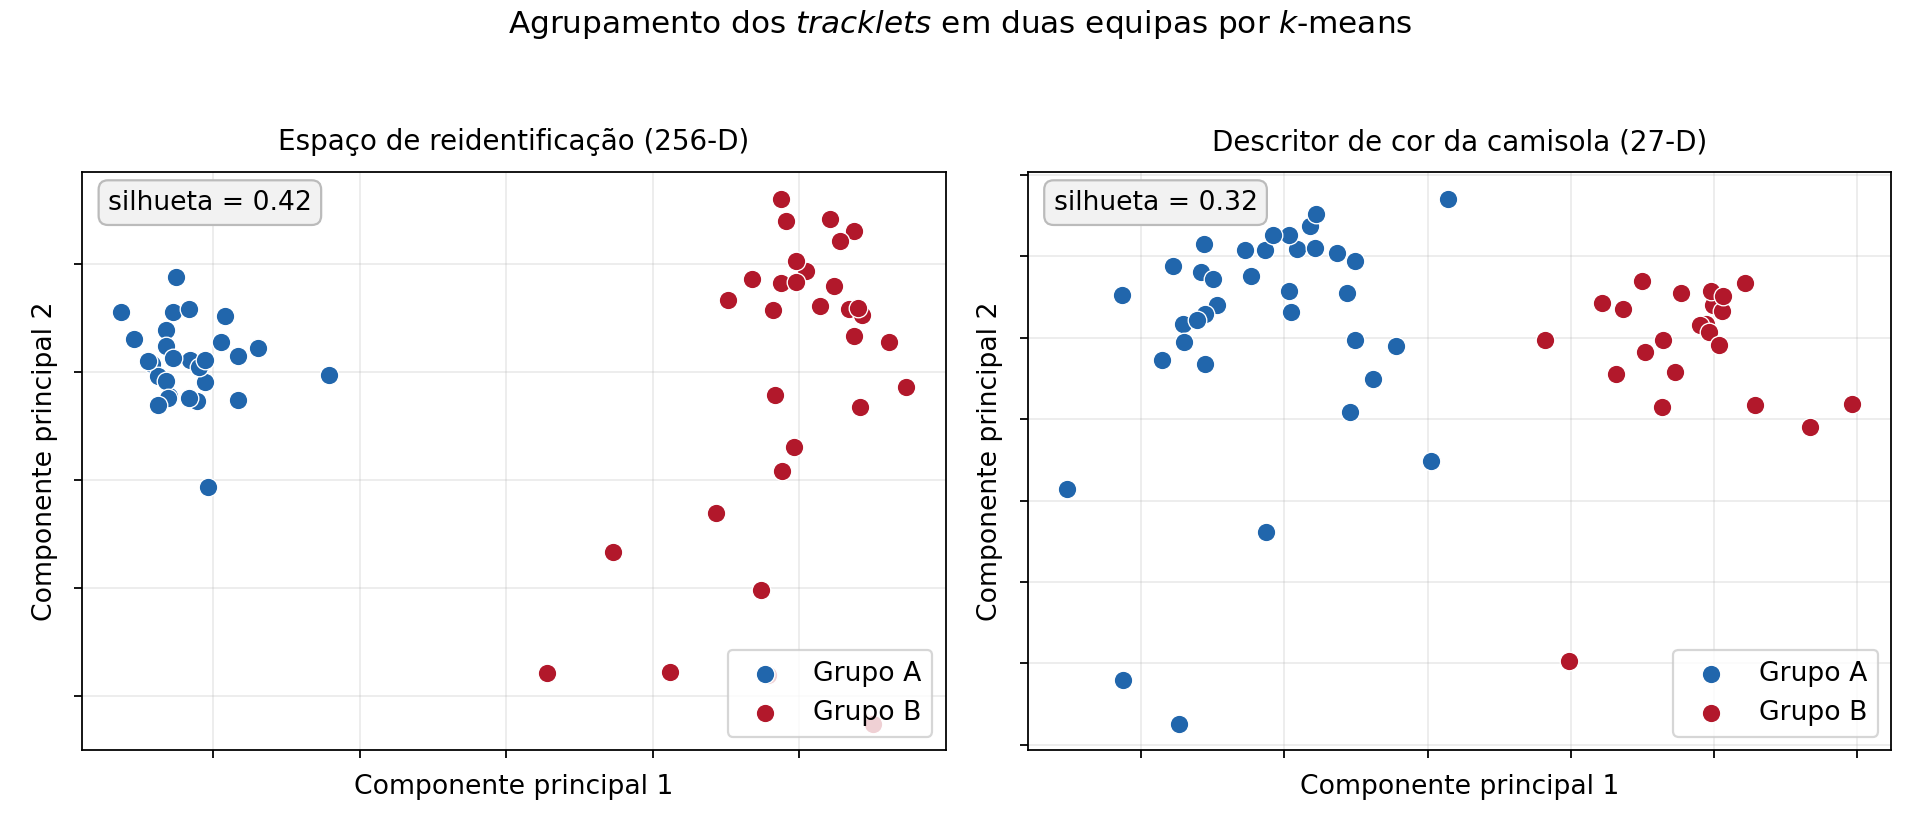
\includegraphics[width=\textwidth]{team_cluster_space.png}
    \caption{Agrupamento dos \emph{tracklets} de um vídeo nas duas equipas. À esquerda, a projeção das características de reidentificação em duas dimensões, onde o \emph{k-means} separa os dois grupos com um coeficiente de silhueta de $0.42$. À direita, o descritor de cor da camisola dos mesmos \emph{tracklets}, que preserva a separação, com silhueta de $0.32$, e serve de alternativa quando a reidentificação é pouco fiável.}
    \label{fig:team_cluster}
\end{figure}

A decisão «Duas equipas?» olha para o resultado, e não para a separação. Aplica-se ao agrupamento que sai da primeira verificação, venha ele da reidentificação ou da cor. Num jogo de futebol há sempre duas equipas em campo, pelo que um agrupamento que deixe quase todas as deteções de jogadores num único grupo está errado, e isso pode ser detetado sem conhecer a anotação. O agrupamento é rejeitado quando o grupo menor fica com menos de $8\%$ das deteções de jogadores. Este limiar não precisou de afinação, porque os dois casos estão bem separados nos dados. Nos vídeos em que a verificação falha, o grupo menor reúne entre $0.1\%$ e $7.8\%$ das deteções, e nos restantes nunca desce abaixo de $8.7\%$.

Um agrupamento rejeitado dá lugar a um reagrupamento pela cor medida diretamente nas imagens, e não pelo descritor da reidentificação. De cada \emph{tracklet} tiram-se $24$ deteções espalhadas ao longo do tempo. Em cada uma recorta-se a parte superior central da caixa, onde fica a camisola, retiram-se os píxeis com cor de relva e calcula-se um histograma HSV com oito intervalos por canal, como na Secção~\ref{sec:descritor-cor}. A média dos $24$ histogramas descreve o \emph{tracklet}, e um \emph{k-means} de dois grupos sobre essas médias dá o agrupamento de resgate. A decisão «Resgate aceite?» impõe duas condições. A primeira exige que o grupo menor tenha pelo menos $20\%$, tanto dos \emph{tracklets} como das deteções, porque um resgate pode repartir bem os \emph{tracklets} e continuar a concentrar as deteções num só grupo. A segunda recusa o resgate quando o classificador de função dá como arbitragem mais de um quarto dos \emph{tracklets} que dá como jogador. Nesse caso falta uma equipa inteira ao agrupamento, e separar por cor o que resta apenas partiria uma equipa ao meio. Se o resgate não for aceite, mantém-se o agrupamento anterior. O efeito desta verificação é medido na Secção~\ref{sec:res_equipa_degenerada}.

A auditoria intervém numa minoria de vídeos. Nos $57$ vídeos de treino, a separação foi dada como pouco clara em $9$. A cor foi aceite em $8$, sete pelo segundo caso e um pelo primeiro, e recusada no nono. Nos $39$ vídeos de teste com estado guardado, a cor foi usada em $4$. A decisão «Duas equipas?» falha em $11$ dos $159$ vídeos, e o resgate é aceite em $8$. Na maioria dos vídeos, portanto, o agrupamento final é o da reidentificação, e é na minoria restante que a cor tem de fazer melhor do que ela.

\subsection{Atribuição do Lado do Campo}\label{sec:mapeamento}

Definidas as duas equipas, falta decidir qual defende a baliza da esquerda e qual defende a da direita. A aparência não diz nada sobre isso, pelo que a única informação disponível é a posição dos jogadores no campo. Todos os critérios, tanto o da \emph{baseline} como os deste módulo, partem da mesma suposição, a de que os jogadores de uma equipa estão, em média, mais perto da sua própria baliza do que os adversários. A \emph{baseline} aplica-a da forma mais direta, comparando a posição média dos dois grupos, como se descreveu no início da Secção~\ref{sec:met-equipa}. Esta comparação tem três fraquezas. Uma única deteção projetada a centenas de metros, por uma falha da calibração, desloca a média do seu grupo. Um jogador que aparece durante todo o vídeo pesa muito mais do que um que aparece pouco. E, sobretudo, quando as duas equipas estão na mesma metade do campo, como em qualquer lance junto de uma baliza, as duas médias ficam a poucos metros uma da outra e a sua ordem deixa de indicar que baliza cada equipa defende.

O módulo reescrito substitui essa comparação por quatro critérios, aplicados por ordem. Cada um tenta decidir o lado e, se não tiver informação suficiente, passa a decisão ao seguinte. Os três primeiros olham apenas para os jogadores de campo, e cada um aceita decidir com menos evidência do que o anterior. O quarto, usado só em último recurso, olha para o guarda-redes. A Tabela~\ref{tab:cascata} resume o que cada critério compara e quando decide.

Todos os critérios usam a posição $x$ dos jogadores no campo, definida na Secção~\ref{sec:agrupamento}, que vai de $-52.5$ metros, na linha de baliza da esquerda, a $+52.5$ metros, na da direita. Todos ignoram as deteções com $|x|$ acima de $60$ metros, isto é, a linha de baliza com uma folga de $7.5$ metros. A folga deixa passar posições reais ou quase, como a de um jogador que fica uns metros para lá da linha depois de um remate, ou a pequena imprecisão da calibração junto às balizas, e elimina apenas as projeções impossíveis, como as de uma falha da calibração que atira os pés para centenas de metros. Fica assim resolvida a primeira fraqueza da média. O valor não foi afinado nos dados. É um número redondo que garante essa folga.

\begin{table}[H]
    \centering
    \caption{Os quatro critérios da cascata, aplicados por ordem até um deles decidir.}
    \label{tab:cascata}
    \small
    \begin{tabular}{|l|p{3.6cm}|p{3.2cm}|p{3.2cm}|}
        \hline
        \textbf{Critério} & \textbf{O que compara} & \textbf{Decide quando} & \textbf{Passa ao seguinte quando} \\
        \hline
        1. Votação por \emph{tracklet} & Em que metade do campo esteve cada \emph{tracklet} & $60\%$ dos \emph{tracklets} de um grupo estão na mesma metade & Os votos estão repartidos, ou os dois grupos ficam na mesma metade \\
        \hline
        2. Votação relativa & A percentagem de \emph{tracklets} de cada grupo na metade direita & As percentagens diferem $10$ pontos ou mais & A diferença é menor \\
        \hline
        3. Posição média & A posição média de cada grupo & As médias distam $0.3$ metros ou mais & As médias quase coincidem e há guarda-redes \\
        \hline
        4. Guarda-redes & Quanto cada grupo avança para a baliza do guarda-redes & Há pelo menos três \emph{tracklets} medidos por grupo & Não há, e decide a posição média \\
        \hline
    \end{tabular}
\end{table}

O primeiro critério olha para onde está cada jogador. Cada \emph{tracklet} conta como um voto, que vai para a metade do campo onde ele esteve, em média. Como se contam \emph{tracklets} e não deteções, um jogador visto durante todo o vídeo deixa de pesar mais do que os outros, o que atenua a segunda fraqueza. Se pelo menos $60\%$ dos votos de um grupo forem para a mesma metade, por exemplo, $12$ de $20$, o grupo fica com esse lado e o outro com o oposto. Num jogo aberto, em que cada equipa ocupa sobretudo a sua metade, este critério decide logo. Não decide quando os votos de um grupo estão repartidos, nem quando os dois grupos têm a maioria na mesma metade, o que acontece sempre que a jogada se passa toda junto de uma baliza.

O segundo critério serve precisamente para quando as duas equipas estão na mesma metade. Mesmo aí, a equipa que defende a baliza da direita costuma ter mais jogadores do lado direito do que a outra. O critério compara, por isso, a percentagem de \emph{tracklets} que cada grupo tem na metade direita. Se um grupo tiver, por exemplo, $70\%$ dos seus \emph{tracklets} à direita e o outro $50\%$, a diferença é de $20$ pontos e o primeiro grupo fica com a direita. Se a diferença for menor do que $10$ pontos, como $52\%$ contra $48\%$, considera-se que não há sinal e passa-se ao critério seguinte. Cada grupo precisa de ter pelo menos três \emph{tracklets}. É uma hipótese razoável na maioria dos lances, mas não é uma regra, e o terceiro exemplo abaixo mostra um caso em que falha.

O terceiro critério é a comparação da \emph{baseline}, agora sem as deteções impossíveis. Calcula-se a posição média de cada grupo, e o que estiver mais à direita fica com a direita. Só não decide quando as duas médias quase coincidem, a menos de $0.3$ metros uma da outra, porque aí a ordem entre elas é ruído. Nesse caso, se houver um guarda-redes detetado, passa-se ao quarto critério.

O quarto critério usa o guarda-redes. Como ele fica junto da sua baliza, a metade em que está indica essa baliza. A equipa que ataca essa baliza aproxima-se dela ao longo do vídeo, ao passo que a equipa que a defende já lá está e pouco avança nessa direção. Mede-se, por isso, quanto cada \emph{tracklet} com pelo menos dez imagens avançou na direção dessa baliza entre a primeira e a última imagem, e faz-se a média por grupo. O grupo que mais avança é o atacante e fica com o lado oposto ao do guarda-redes, e o outro, a equipa do guarda-redes, fica com o lado dele. Se algum grupo tiver menos de três \emph{tracklets} assim medidos, decide a posição média. Os próprios guarda-redes recebem, como na \emph{baseline}, o lado da metade em que se encontram.

Experimentou-se ainda uma quinta regra, que dava como atacante o grupo mais próximo de uma baliza numa bola parada. Foi retirada porque, nos $39$ vídeos de teste, disparou uma vez e errou, já que o grupo que se junta perto de uma baliza é, pelo menos com a mesma frequência, o que a defende.

A Figura~\ref{fig:cascata-exemplos} mostra a cascata em três vídeos reais, em que A e B são os dois grupos que saem do agrupamento. No SNGS-060, o caso mais comum, o jogo está aberto e as equipas repartem-se pelas duas metades. Nenhum grupo chega aos $60\%$ na votação por \emph{tracklet}, a votação relativa fica nos $8$ pontos e é a comparação de médias que decide, com $4.4$ metros de diferença e corretamente. No SNGS-195, o jogo decorre inteiro na metade esquerda e as médias dos dois grupos ficam a um centímetro uma da outra. Decide o guarda-redes, junto da baliza esquerda. O grupo B avançou em média $5.8$ metros na direção dessa baliza e o grupo A apenas $1.4$, pelo que B é o atacante e recebe \emph{right}. Os $31$ \emph{tracklets} do vídeo ficam corretos, quando antes deste critério ficavam todos errados.

\begin{figure}[H]
    \centering
    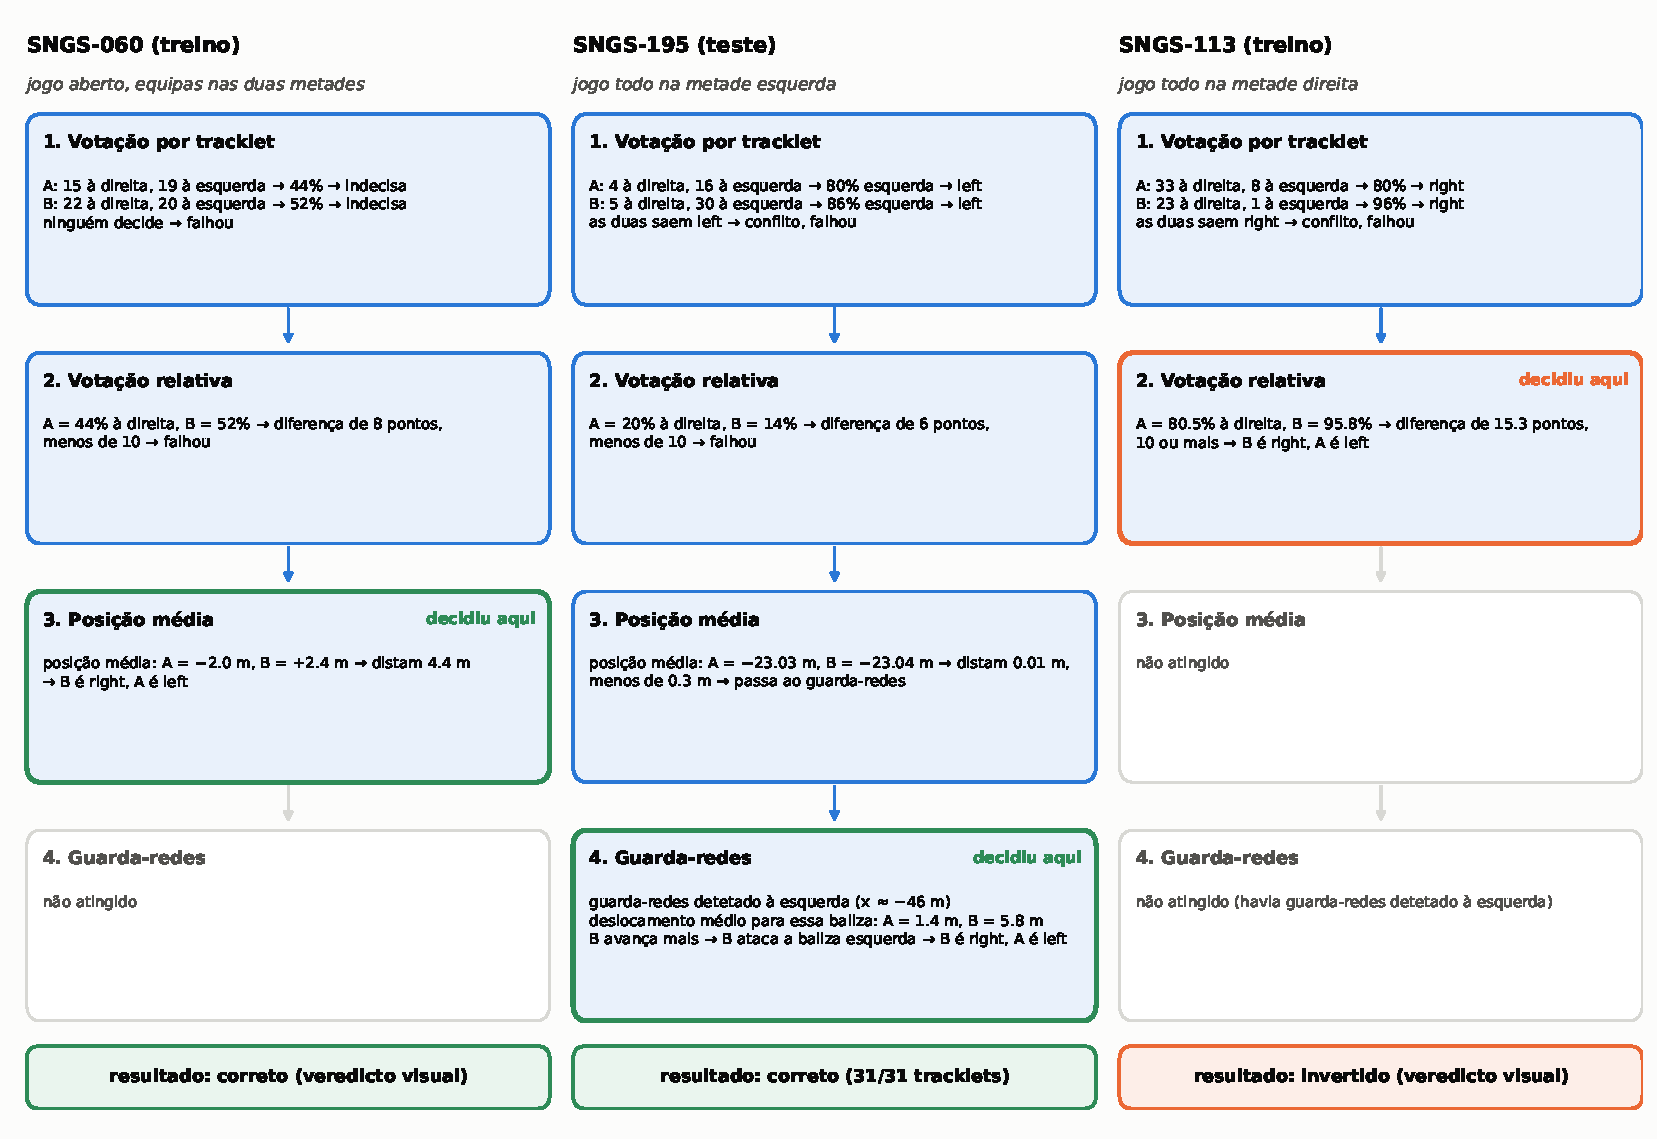
\includegraphics[width=\textwidth]{fig_cascata_exemplos.pdf}
    \caption{A cascata do lado em três vídeos reais, com o critério que decide em cada um e o resultado.}
    \label{fig:cascata-exemplos}
\end{figure}

O SNGS-113 mostra onde a cascata falha. As duas equipas estão na metade direita, com as medianas a apenas $9.7$ metros uma da outra, ao passo que os guarda-redes distam $73.5$ metros (Figura~\ref{fig:113-campo}). Os dois grupos têm a maioria dos \emph{tracklets} na metade direita, $80.5\%$ e $95.8\%$, pelo que a votação por \emph{tracklet} não decide. A votação relativa decide pela diferença de $15.3$ pontos e dá o lado direito a B. O resultado está invertido. Essa diferença corresponde a oito \emph{tracklets} contra um do lado esquerdo, num vídeo com $65$ \emph{tracklets} para cerca de vinte jogadores. São fragmentos de trajetórias, e um jogador que o \emph{tracking} partiu em vários pedaços conta várias vezes. Com as duas equipas na mesma metade, essa diferença é ruído e não um sinal do lado. O guarda-redes, que resolveria o caso sem ambiguidade, só é consultado no fim, e o segundo critério decide antes.

\begin{figure}[H]
    \centering
    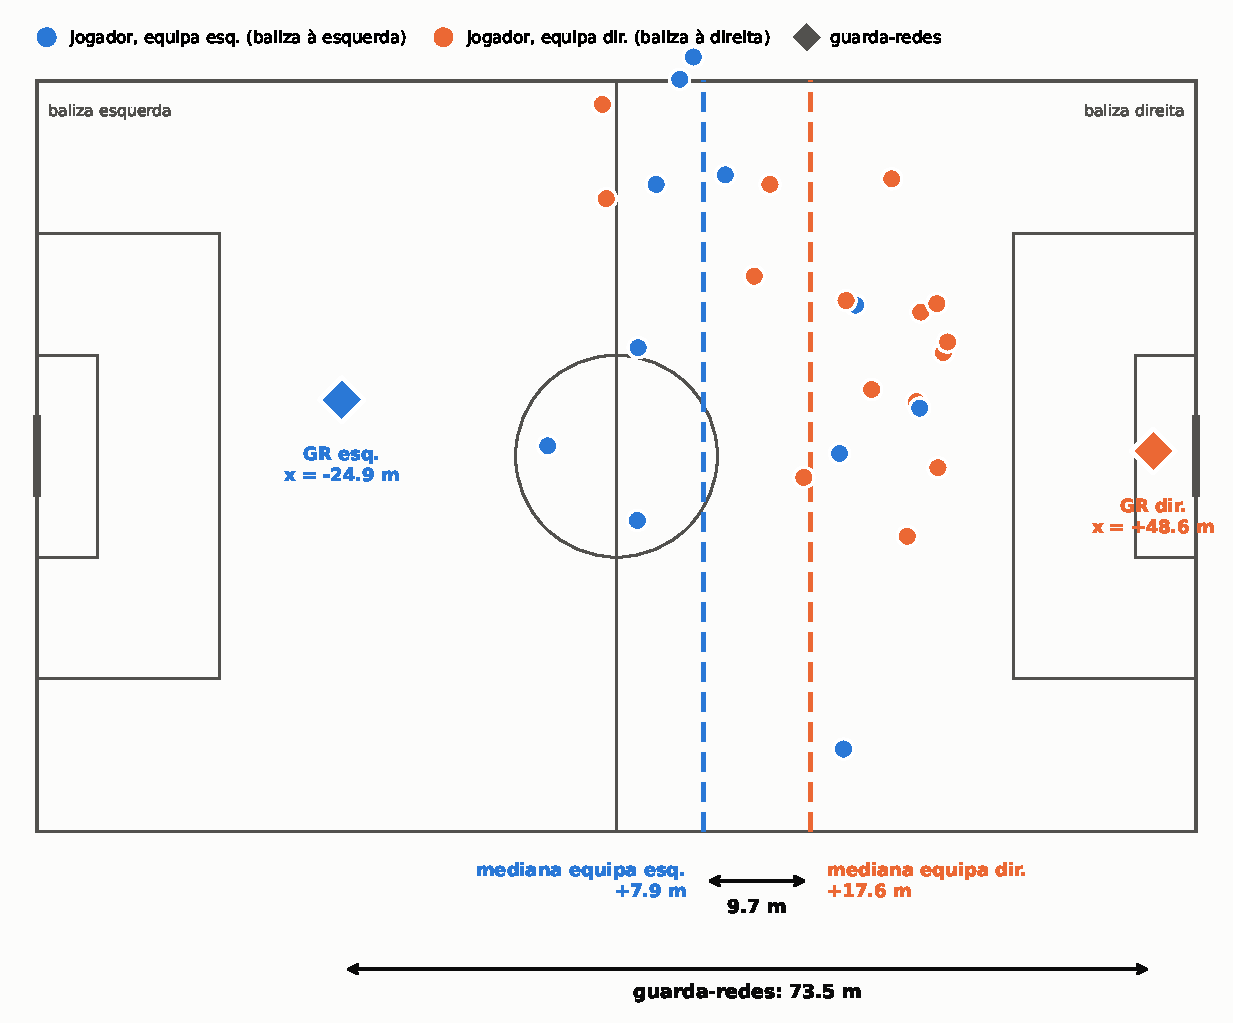
\includegraphics[width=0.9\textwidth]{fig_113_campo.pdf}
    \caption{Anotação de referência do SNGS-113, com a posição mediana de cada jogador. As duas equipas estão na mesma metade e os guarda-redes nos extremos.}
    \label{fig:113-campo}
\end{figure}

A frequência com que cada critério decide mostra que o guarda-redes quase nunca chega a ser consultado. Nos $57$ vídeos de treino, a decisão saiu do primeiro critério em $17$, do segundo em $12$, do terceiro em $28$ e do quarto em nenhum. Nos $39$ vídeos de teste com estado guardado, saiu do primeiro em $5$, do terceiro em $33$ e do quarto em $1$. Na maioria dos vídeos decide, portanto, a comparação de médias da \emph{baseline}, agora protegida pelo filtro dos $60$ metros, e as votações só decidem quando as equipas estão claramente em metades diferentes ou há uma assimetria de pelo menos $10$ pontos. O Capítulo~\ref{cap:resultados} mede, vídeo a vídeo, onde a cascata corrige a \emph{baseline}. O guarda-redes, o sinal mais fiável para esta decisão por não acompanhar as fases de ataque, continua em último lugar, e passá-lo para a frente da cascata fica como a alteração com mais potencial por fazer.

Os limiares da cascata foram recalibrados sobre os conjuntos de teste e de validação em conjunto. A maioria exigida na votação por \emph{tracklet} é de $60\%$, a diferença mínima da votação relativa desceu de $25$ para $10$ pontos e a distância mínima entre médias desceu de $0.5$ para $0.3$ metros. Cada ajuste só foi aceite se resolvia vídeos que falhavam sem estragar nenhum dos que já estavam corretos no conjunto de teste.

\FloatBarrier

\section{Ambiente Experimental}

Esta secção descreve as condições em que o sistema foi desenvolvido e avaliado. Apresenta o ambiente computacional e o conjunto de dados, enumera os hiperparâmetros que governam os módulos alterados e define o procedimento de avaliação sobre o qual assentam os resultados do capítulo seguinte.

\subsection{Ambiente Computacional e Conjunto de Dados}\label{sec:ambiente}

Todo o trabalho foi implementado com base no \emph{framework} TrackLab, responsável pela gestão e execução sequencial dos módulos do \emph{pipeline}, tendo como suporte a biblioteca PyTorch \citep{paszke2019pytorch}. O desenvolvimento decorreu em Python~3.10. A avaliação final, tanto do sistema proposto como da \emph{baseline}, correu num único ambiente em Python~3.12, com as versões das bibliotecas fixadas, de modo que os dois sistemas são comparados nas mesmas condições. A principal restrição computacional decorreu da infraestrutura de \emph{hardware} disponível, um sistema portátil equipado com uma GPU NVIDIA RTX~3060 com apenas 6~GB de VRAM. Esta limitação condicionou várias das decisões metodológicas adotadas, com destaque para a quantização a 4 bits, com recurso à biblioteca \emph{bitsandbytes}, do modelo de visão e linguagem responsável pela leitura do número da camisola (Qwen2.5\babelhyphen{nobreak}VL\babelhyphen{nobreak}3B), e para a gestão explícita da memória de vídeo entre sequências. Como os módulos partilham a mesma GPU, o modelo de visão e linguagem é libertado no fim de cada vídeo. Assim, os pontos do campo e a calibração do vídeo seguinte, que correm antes dele, têm memória disponível. O modelo volta depois a ser carregado do disco, em cerca de cinco segundos.

A avaliação usou o conjunto de dados SoccerNet-GSR, formado por sequências de vídeo de 30 segundos, todas anotadas e divididas em três subconjuntos. São 160 sequências, 57 de treino, 54 de validação e 49 de teste. Uma delas, o SNGS-096 da validação, não pôde ser processada, porque o módulo de calibração falha nesse vídeo nos dois sistemas. A comparação incide, por isso, sobre 159 vídeos. Em cada \emph{frame}, a anotação de referência (\emph{ground truth}) indica a posição de cada interveniente no campo, a sua equipa, a função e o número da camisola. Isto permite avaliar o sistema completo e também cada módulo isoladamente.

O papel de cada subconjunto neste trabalho difere do habitual. Nenhum dos módulos desenvolvidos obriga a treinar modelos, pelo que o subconjunto de treino não foi usado para aprender parâmetros. As regras e os limiares de decisão foram escolhidos sobre os conjuntos de teste e de validação, como se descreve na Secção~\ref{sec:mapeamento}. O conjunto de treino serviu apenas para confirmar cada alteração depois de tomada a decisão. Não é, ainda assim, um conjunto nunca visto. Os seus vídeos foram inspecionados visualmente, como os restantes, e alguns servem de exemplo neste capítulo. A verificação do agrupamento colapsado foi, além disso, desenhada já com os 159 vídeos avaliados. Os resultados do treino mostram, por isso, que as regras se mantêm em vídeos que não serviram para as escolher, mas não equivalem a uma avaliação totalmente cega.


\subsection{Parametrização dos Módulos}

O comportamento dos módulos desenvolvidos é definido por um conjunto de hiperparâmetros, resumidos na Tabela~\ref{tab:hiperparametros}. Os valores relativos ao reconhecimento do número da camisola foram definidos por experimentação, para equilibrar a fiabilidade da leitura com o custo computacional. O limiar de confiança foi escolhido com o GS-HOTA oficial (Secção~\ref{sec:res_jnr_confianca}). Os limiares da atribuição da equipa e do lado do campo resultam da recalibração descrita na Secção~\ref{sec:mapeamento}, conduzida sobre os conjuntos de teste e de validação.


\begin{table}[htbp]
    \centering
    \caption{Hiperparâmetros dos módulos alterados e respetiva função.}
    \label{tab:hiperparametros}
    \footnotesize
    \setlength{\tabcolsep}{4pt}
    \renewcommand{\arraystretch}{0.95}
    \begin{tabular}{|l|l|l|}
        \hline
        \textbf{Parâmetro} & \textbf{Valor} & \textbf{Função} \\
        \hline
        \multicolumn{3}{|l|}{\emph{Reconhecimento do número da camisola (pose e recorte)}} \\
        \hline
        Confiança da pose            & $0.25$          & Deteção mínima dos \emph{keypoints} \\
        \hline
        Alargamento lateral da ROI   & $0.55$          & Margem lateral sobre o tronco \\
        \hline
        Margem superior da ROI       & $0.10$          & Recorte acima dos ombros \\
        \hline
        Fração de altura do tronco   & $0.90$          & Extensão vertical da região dorsal \\
        \hline
        \multicolumn{3}{|l|}{\emph{Reconhecimento do número da camisola (filtro de qualidade)}} \\
        \hline
        Dimensão mínima do recorte   & $15\times20$~px & Rejeita jogadores muito distantes \\
        \hline
        Nitidez mínima               & $15.0$          & Variância do Laplaciano \\
        \hline
        \multicolumn{3}{|l|}{\emph{Reconhecimento do número da camisola (leitura e decisão)}} \\
        \hline
        Modelo de leitura            & Qwen2.5-VL-3B (4 bits) & Inferência do número \\
        \hline
        Recortes por janela          & $6$             & Unidade de decisão temporal \\
        \hline
        Recortes lidos por janela    & $5$             & Os mais nítidos da janela \\
        \hline
        Confiança mínima para votar  & $0.5$           & Produto das probabilidades dos \emph{tokens} \\
        \hline
        \multicolumn{3}{|l|}{\emph{Descritor de cor (reidentificação)}} \\
        \hline
        Atenção mínima do torso      & $0.25$          & Valor mínimo no mapa do tronco do PRTreID (0--1) \\
        \hline
        Píxeis mínimos da máscara    & $16$            & Abaixo, usa a banda central \\
        \hline
        Classes por canal HSV        & $8$             & Três canais, $24$ valores \\
        \hline
        \multicolumn{3}{|l|}{\emph{Atribuição da equipa (agrupamento)}} \\
        \hline
        Limiar de silhueta           & $0.28$          & Abaixo, recorre à cor da camisola \\
        \hline
        Concentração num dos lados   & $0.85$          & Condição do teste complementar \\
        \hline
        Distância entre centros      & $2.04$          & Abaixo, separação por ReID frágil \\
        \hline
        Fração mínima do grupo menor & $0.20$          & Aceitação da alternativa de cor, em \emph{tracklets} e em deteções \\
        \hline
        Dimensão do descritor de cor & $27$            & $24$ do histograma HSV e $3$ da média Lab \\
        \hline
        Deteções mínimas do grupo menor & $0.08$       & Abaixo, partição degenerada e reagrupamento \\
        \hline
        Recortes por \emph{tracklet} (resgate) & $24$  & Amostra uniforme no tempo \\
        \hline
        Região do tronco (resgate)   & $0.6 \times 0.4$ & Fração central da caixa, largura e altura \\
        \hline
        Razão máxima árbitros/jogadores & $0.25$       & Acima, falta uma equipa e não se reagrupa \\
        \hline
        Posição válida (agrupamento) & $|x| \le 52.5$~m & Ignora projeções fora do relvado \\
        \hline
        \multicolumn{3}{|l|}{\emph{Atribuição da equipa (lado do campo)}} \\
        \hline
        Posição válida (lado)        & $|x| \le 60$~m   & Descarta artefactos de calibração \\
        \hline
        Maioria na votação           & $0.60$          & Fração dominante por \emph{tracklet} \\
        \hline
        Diferença relativa mínima    & $0.10$          & Margem do voto relativo \\
        \hline
        Distância mínima entre médias & $0.3$~m        & Abaixo, aciona o desempate pelo guarda-redes \\
        \hline
        Imagens mínimas por \emph{tracklet} & $10$    & Para medir o deslocamento no desempate \\
        \hline
    \end{tabular}
\end{table}


\FloatBarrier
\subsection{Procedimento de Avaliação}\label{sec:protocolo}

A avaliação foi feita em dois níveis, conforme se descreveu na Secção~\ref{sec:metricas}. Para o sistema completo, isto é, com todos os módulos, o desempenho é avaliado e medido pela métrica oficial do desafio, o GS-HOTA. Contudo, para separar o contributo de cada módulo, a métrica é recalculada por fases. Começa-se só com a posição e vai-se juntando, uma de cada vez, a função, a equipa e o número da camisola. Cada atributo que se acrescenta faz a métrica descer, e o tamanho dessa descida mede quanto esse atributo, e logo o módulo que o produz, custa ao resultado final.

O termo de comparação é a \emph{baseline} executada no ambiente de desenvolvimento descrito acima, nos mesmos 159 vídeos, com os módulos originais. Como a deteção, o \emph{tracking} e as representações de reidentificação são partilhados, os \emph{tracklets} avaliados são os mesmos nos dois sistemas e qualquer diferença resulta apenas dos módulos alterados. Para além das métricas automáticas, incluiu-se a inspeção visual dos 159 vídeos de cada sistema, em que cada vídeo é classificado como correto, com o lado trocado, com o agrupamento colapsado numa só equipa, com o agrupamento misturado ou com uma equipa inteira classificada como árbitros. Esta inspeção serve para caracterizar os erros que a métrica agrega e para identificar os vídeos em que a própria anotação de referência está invertida.

A recalibração dos limiares da equipa e do lado seguiu uma regra simples. Cada alteração foi testada nos conjuntos de teste e de validação e só foi aceite se corrigia vídeos que falhavam sem estragar nenhum que a versão anterior já acertava. Esta regra compara cada versão com a anterior e não com a \emph{baseline}. Por isso, o sistema final ainda fica abaixo da \emph{baseline} em 11 vídeos, cinco deles do bloco da equipa de amarelo, como se analisa na Secção~\ref{sec:res_equipa_regressoes}. O conjunto de treino, que não entrou nestes ajustes, permite verificar se os ganhos se mantêm fora dos vídeos usados para os obter.